\documentclass[12pt]{article}
\usepackage{/home/sci/weiliu/haldefs}
\usepackage{graphicx}
\usepackage{url}
\usepackage{textcomp}
\usepackage{enumitem}
\usepackage{subfig}
\usepackage{hyperref}
\usepackage{verbatim}
\usepackage{amsmath}
\usepackage{verbatim}
\usepackage{natbib}
\usepackage{algorithmic}
\usepackage{algorithm}
\usepackage{color}
\usepackage{mdwlist}

\hypersetup{
  % bookmarks=true,         % show bookmarks bar?
    unicode=false,          % non-Latin characters in Acrobat’s bookmarks
    pdftoolbar=true,        % show Acrobat’s toolbar?
    pdfmenubar=true,        % show Acrobat’s menu?
    pdffitwindow=false,     % window fit to page when opened
    pdfstartview={FitH},    % fits the width of the page to the window
    pdftitle={Reading notes},
    pdfauthor={Wei Liu},     % author
    pdfsubject={Reading notes},   % subject of the document
    pdfcreator={Wei Liu},   % creator of the document
    pdfproducer={Producer}, % producer of the document
    pdfkeywords={reading, papers, functional MRI, connectivity}, % list of keywords
    pdfnewwindow=true,      % links in new window
    colorlinks= true,       % false: boxed links; true: colored links
    linkcolor=blue,          % color of internal links
    citecolor=blue,        % color of links to bibliography
    filecolor=magenta,      % color of file links
    urlcolor=cyan           % color of external links
}


\setlength{\oddsidemargin}{0 in}
\setlength{\evensidemargin}{0 in}
\setlength{\topmargin}{-0.6 in}
\setlength{\textwidth}{6.5 in}
\setlength{\textheight}{9 in}
\setlength{\headsep}{0.5 in}
\setlength{\parindent}{0 in}
\setlength{\parskip}{0.1 in}



\begin{document}
\title{Notes for Revision of Journal Paper}
\author{Wei Liu}
\maketitle

\section{HMRF and Phenotype (Age, Sex)}
The first reviwer has a comment about the possible impact of HMRF regularization
on the individual subject's difference of the variables of interest, such as age
and sex. Such impact happens only when the functional patterns of the subjects
is correlated with the phenotype variables. 

\subsection{Age}
In order to test the relationship between the functional connectivities and the
age, I use Power's selection of ROIs (264 seeds) and computed the pairwise
correlation matrices for all subjects. The total number of pairwise correlation
is $264 \times 263 / 2 = 34716$. I run a T test on each element of the matrix over
all subjects (25), to see if the correlation is significantly different between
male (10) and female (15) group. To take into account the multiple comparison
problem, I use FDR to correct the p values computed from the T test. The result
shows no correlation in the 34716 experiments has a p value less than 0.05. This
result indicates that there is no significant correlation between the functional
connectivities estimated by linear correlation and the sex variable. Therefore,
our HMRF model does not have the risk of diminishing the individual's difference
with regard to the sex variable.

Need to test label maps. For age, use logistic regression and for sex, use
contingence tables (M/F, 0/1) and Fisher exact test. Choose a voxel with both 0
and 1 variables (balanced. )

To test the correlation between the binary network label variables and the
\textsf{age} variables, I select those voxels with at least 20 percent of zeros
or 20 percent of ones for the binary network labels. For DMN, the resultant
number of voxels is 8321. For each voxel, I did a logistic regression using 25
subjects as samples, and save the coefficients. The logistic regression is done
for the network labels estimated from both the non-hierarchical models (K-Means)
and HMRF model. Then we obtain two coefficients at each voxel. 

Next, we are interested in whether the coefficients of the logistic regression
for the HMRF is different from the coefficients for the non-hierarchical
model. If we assume the difference of the two coefficients at each voxel are
i.i.d Gaussian, we can use t test to test the hypothesis that there is no
difference between the two coefficients.

Note the i.i.d assumption of the coefficients may not be a valid one. 

Figure \ref{fig:coe_density_dmn} shows the histograms of the coefficients of all
8321 voxels extracted from the DMN network. It can be seen the coefficients
estimated from the hierarchical model is less than the non-hierarchical
model. This is difficult to interpret. I also did a paired t test on the
coefficients of two models. The null hypothesis is the mean coefficients are
equal, and the alternative is the non-hierarchical coefficients are greater than
the coefficients of HMRF. The t test also shows the significant difference
between the mean coefficients of two models.

After the discussion with Tom, to test whether the regression coefficients shift
towards zero for the HRMF model, I subtract the mean from the coefficients of
both hierarchical and non-hierarchical model, and square the coefficients. The
histogram of the squared coefficients are shown in Fig.
\ref{fig:coe2_hist_dmn}. We use F test to see if $\beta_1^2 / \beta_2^2$ is
different from 1. The result of the F test (\textsf{var.test} command in R)
shows p value = 0.13, which means the $\beta_1^2$ and $\beta_2^2$ is not
significantly different. Therefore, our hierarchical model shifts the regression
coefficients to the left side as can be shown by the t test, but the
hierarchical model does not result in smaller variance of the coefficients,
shown by the F test.

However, when repeating the same F test on attentive network (network label 3 in
current label maps), the F test shows the $\beta$ from hierarchical model has
significantly greater than the non-hierarchical model. The estimate F ration is
0.8.

When repeating the F test on visual network (network label 1), $\cF =
1.147$. The $\beta$ of hierarchical model is smaller.

\begin{figure}[htb]
  \centering
  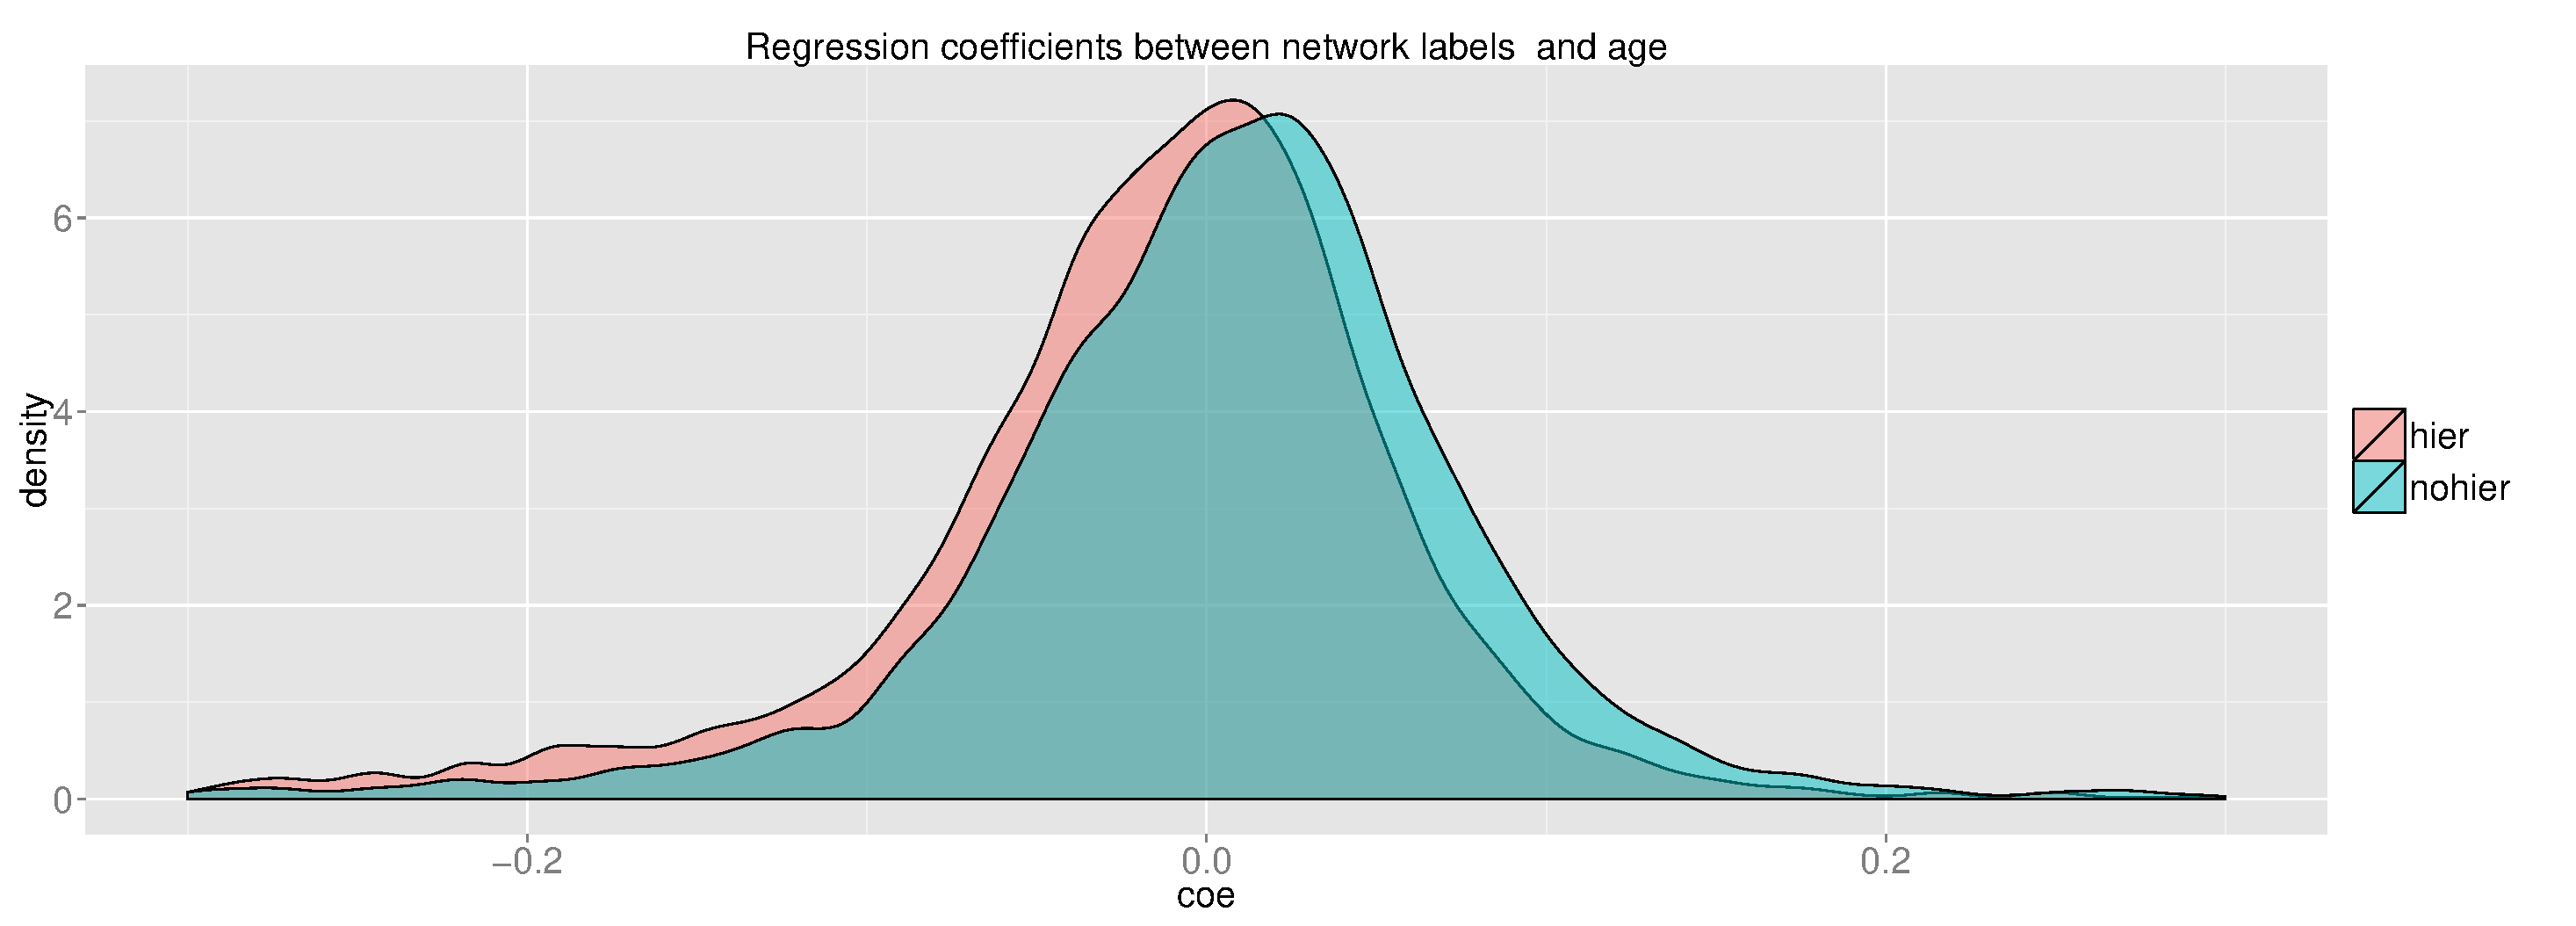
\includegraphics[width = 1.0\textwidth]{figures/coe_density_dmn}
  \caption{ Density estimation from the histogram of the coefficients of the
    logistic regression between DMN binary labels and \textsf{age} variables for
    both non-hierarchical (K-Means) and HMRF model.}
  \label{fig:coe_density_dmn}
\end{figure}

\begin{figure}[htb]
  \centering
  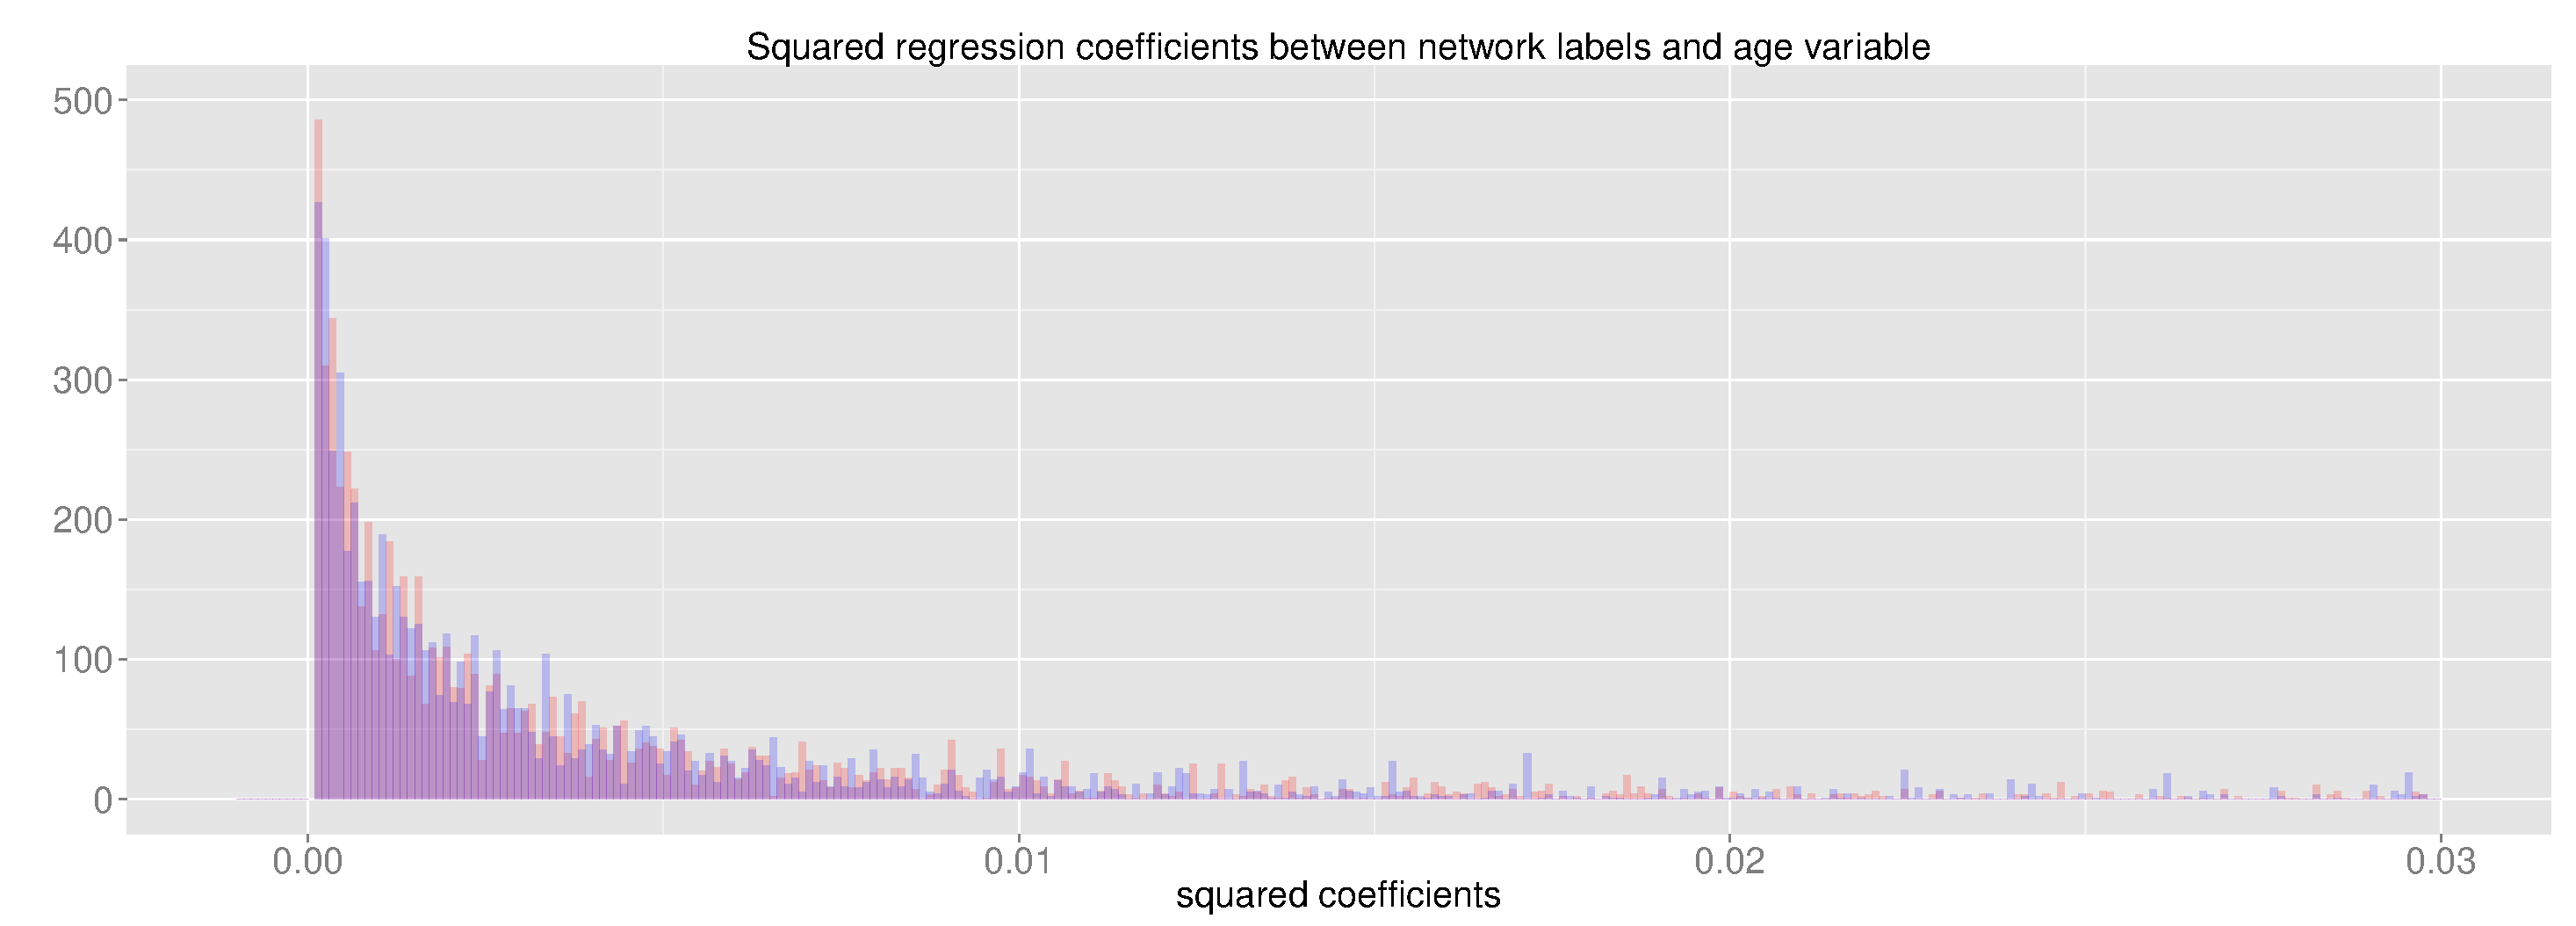
\includegraphics[width = 0.9\textwidth]{figures/coe2_hist_dmn} \\
  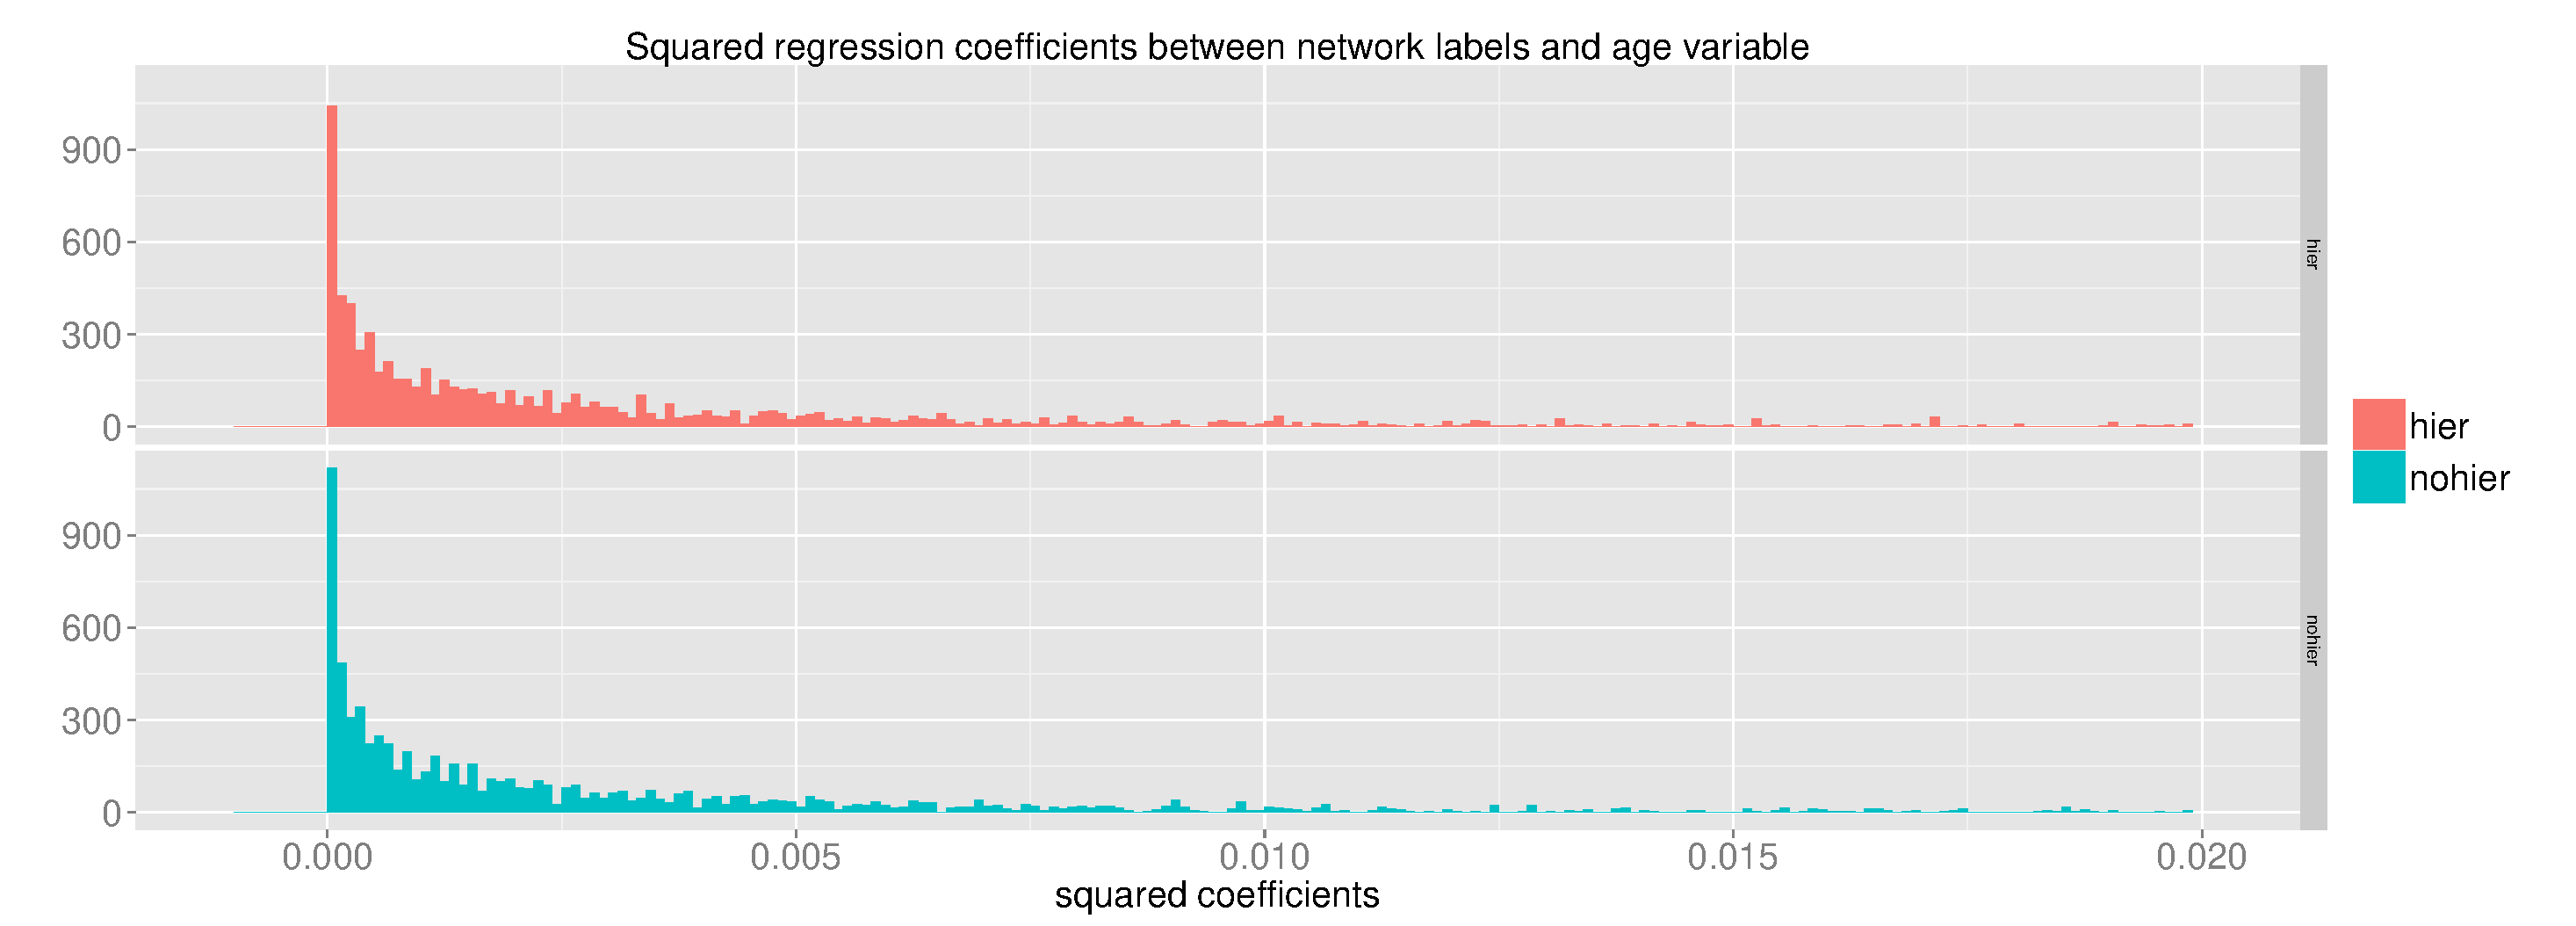
\includegraphics[width = 0.9\textwidth]{figures/coe2_hist2_dmn}
  \caption{ Histogram of the squared coefficients of the logistic regression
    between the binary labels of DMN and \textsf{age} variables for both
    non-hierarchical (K-Means) and HMRF model. The squared coefficients is
    computed after subtracting the mean of the coefficients. Top figure gives
    overlapped histograms, and bottom shows the two histograms side by side.}
  \label{fig:coe2_hist_dmn}
\end{figure}

After the discussion with Tom on 6/1, discard the single F test. Now on DMN, for
the non-hierarchical model, select 8321 voxels for logistic regression. Then use
wald test to find the p value of the regression coefficients. With FDR
correction, there are 469 voxels has significance > 0.05. With FDR correction,
not a single voxel is significant at 0.1. For the hierarchical model, the number
of voxels with non-zero coefficients at the same $\alpha = 0.05$ is 352. Compare
469 and 352, it seems to show that hierarchical model decreases the possible
non-zero coefficients.

Repeating the above experiment with attentive network (label 3), from total 6398
voxels, non-hierarchical model have 371 voxels significant, and hierarchical
model has 199.

Repeating the above experiment with visual network (label 1): from total 4093
voxels, non-hierarchical model has 195 significant voxels, and HMRF has 170.

Motor (label 2): total 7366 voxels. Non-hier: 251 significant. Hier: 412.

Salience (label 4:) total 3580. Non-hier: 253 significant. Hier: 289. 

Executive control (label 6) total 8715.  non-hier: 563. Hier: 743. 

\begin{figure}[htb]
  \centering
  \includegraphics[width = 0.4\textwidth]{/home/sci/weiliu/projects/hmrf_journal/revision/phenotypes/dmn/coeff_nohier}
  \includegraphics[width = 0.4\textwidth]{/home/sci/weiliu/projects/hmrf_journal/revision/phenotypes/dmn/coeff_hier}
  
\includegraphics[width = 0.03\textwidth]{/home/sci/weiliu/projects/hmrf_journal/menuscript/figures/autumn_bar}
  \caption{The logistic regression coefficients for DMN of non-hierarchical
    model (K-Means, left figure) and hierarchical model (HMRF, right). The
    binary label map of DMN is extracted from all subjects. A subset of gray
    matter voxels is selected such that the voxel includes both 0 (out network)
    and 1's (in network) across 25 subjects. Color map ranges (-0.2,
    0.2). voxels outside the range are not shown. }
\end{figure}


\subsection{Sex}
To test the effect of hierarchical model on the possible correlation between sex
and functional networks, I made a contingency table of sex and the binary
labels, and compute the $\chi^2$ statistics at each voxel. The Prearson's
$\chi^2$ statistics tests whether the two variables, sex and network labels, are
independent. Under the null hypothesis of independence, the statistics is
approximately a $\chi^2$ distribution. The $\chi^2$ statistics is calculated by
averaging the ratio $ (O - E) / E $ over all columns and rows, where $O$ is the
observed frequency and $E$ is the expected frequency. A larger value will result
in the rejection of the null hypothesis. 

We save the $\chi^2$ statistics at each voxel for non-hierarchical and
hierarchical model specifically. Then, a F test is used to test if the ratio of
$\chi^2$ of hierarchical and non-hierarchical model are equal to one. We can use
F test, because
\[
\cF_{a, b} = \frac{\chi_a^2 / a}{\chi_b^2 / b}
\]
% http://flower.amath.nchu.edu.tw/web/member/room/605Lecture/Lecture%2005_addendum_Chisquare,t%20and%20F%20distributions.PDF
is a F distribution. Here $\chi_a^2 = \sum_n \chi_n^2$ is from non-hierarchical
model, and $\chi_b^2 = \sum_n \chi_n^2$ is from hierarchical model. Because our
input data is the $\chi^2$ statistics that we calculated from the contingency
table, we can not simply use \textsf{var.test} function of R to do the F
test. Instead, we need to explicitly compute $\chi_a^2$ and $\chi_b^2$, and the
ratio of them as the $\cF_{a,b}$ statistics. The degree of freedom $a$ and $b$
are same, and equal to $(r-1)(c-1)$, where $r$ and $c$ are the row and column
number in the contingency table. In our case, $r = c = 2$ for male/female and
in/out network, so $a = b = 1$.

The F test result is surprising. $\cF_{a,b} = 0.832$, which means the average
$\chi^2$ of hierarchical model is greater than the non-hierarchical model. By
the definition of the $\chi^2$ test of the contingency table, a large value of
$\chi^2$ means less possibility of independence between sex and network
labels. This result is different from the F test on the age. Since the
hierarchical model estimates networks that are more similar across subjects,
ideally the binary network labels should be less dependent on both the age and
the sex variable, if there is any dependency. 

However, when repeating the above test on attentive network, the F ratio
$\cF_{a,b} = 1.216$, which means the average $\chi^2$ of the hierarchical model
is less than the non-hierarchical model. Therefore, there are less dependency
between sex and network labels for the hierarchical model.

When repeating the test on visual network, $\cF = 0.6$, indicating label maps
estimated by hierarchical model has greater dependency on the sex variable. 

Since the total number of subjects are 25, a small number, $\chi^2$ test may not
be a good test since the $\chi^2$ statistics is approximately in $\chi^2$
distribution. Other methods, such as likelihood ratio $\chi^2$ test, or Fisher's
exact test, might be better
alternatives\footnote{http://www.uvm.edu/~dhowell/methods7/Supplements/ChiSquareTests.pdf}.

Overall, the correlation with age and sex change with the hierarchical model in
an unpredictable way. For some functional networks, the correlation are
stronger, and for others, they are weaker. 


After the discussion with Tom on 1/6, we conclude the current method is not
good. We should plot a map of the regression coefficients for both age and sex
variables. Then, we should count the significant voxels with or without
hierarchical model, and see if the number of significant voxels change.


\begin{figure}[htb]
  \centering
  \includegraphics[width = 1.0\textwidth]{/home/sci/weiliu/projects/hmrf_journal/revision/phenotypes/dmn/dmn_sex_hist}
  \caption{The histogram of the $\chi^2$ statistics for non-hierarchical
    (K-Means) and hierarchical model (HMRF). }
\end{figure}

A $\chi^2$ test on the (sex, DMN network) contingency table shows no significant
voxels after FDR correction. Without FDR correction, non-hierarchical model has
148 voxels significant, and hierarchical model has 185 significant. This
indicates hierarchical model, surprisingly, increases the dependency of the sex
and DMN network.

A Fisher's test on the same contingency table shows that non-hierarchical model
has 79 significant voxels, while the hierarchical model has 106.


Test on attentive network (6398 voxel in total): Fisher test shows
non-hierarchical model: 164. Hierarchical: 112. $\chi^2$ test shows non-hier:
138. hier: 58.

Test on visual network (4093): $\chi^2$ test, non-hier: 47, hier: 165. Fisher
test, non-hier: 140. hier: 259.

Test on motor (7366 voxels): $\chi^2$ test, non-hier: 165, hier: 68. Fisher
test, non-hier: 333. hier: 126.

Test on salience (3580 voxels): $\chi^2$ test, non-hier: 51, hier: 70. Fisher
test, non-hier: 74 . hier: 134.

Test on executive control (8715 voxels): $\chi^2$ test, non-hier: 127, hier: 151. Fisher
test, non-hier: 96. hier: 227.




\section{Comparison with ICA}
One critical comment from the second reviewer is to compare the HMRF model with
ICA. In the current experiments, there are inter-session test and bootstrap
test. We do not need (or have time) to test ICA on both. If we test ICA on the
inter-session consistency, There are two possible options

\begin{itemize}
  \item We can follow what we have done in 2011 MICCAI workshop paper, and
    extract a binary map for each functional network by group ICA method
    (temporal ICA in Gift package). For each subject, each session and each
    network, we get a binary label map. We then compute the variance across the
    3 sessions for each network, just like the current 0-1-2 map of HMRF
    method. However, such variance map is just for one network. We need an
    additional step to aggregate the variance map over all networks in order to
    compare with HMRF, since HMRF has a single variance map for all networks. We
    can simply average the variance over all networks.

    One possible issue with this method is, after averaging over all components,
    the variance will by very small. This is because for a particular voxel,
    most of the components are just constant, and the icc value will be zero. So
    a smaller number of non-zero icc, combined with large number of zero icc,
    will have a small average value. This average value may not reflect the true
    variance of the ICA method.

    \item We can follow the NYU TRT work of Zuo, and use ICC to test the
      inter-session consistency per voxel. Since ICC works for continuous
      values, there is no need to threshold the ICA component map. Each voxel
      has a Jx3 matrix for each ICA component, where J is the number of
      subjects. Because HMRF variance is over all clusters, the ICC should be
      averaged over all ICA components. Such averaging is an empirical approach.
\end{itemize}

Now I have the results of the second option above, i.e. average ICC map over all
ICA components. Since ICC is in $(-1,. 1)$ and large value means better
consistency between sessions, so it is in the opposite trend with our existing
0-1-2 map. We may need a $1 - ICC$ value for better comparison with existing
variance maps. But even after this conversion, the ICC value still can not be
compared with variance map, as they are different metric. 

After the discussion with Tom on 1/6, we decide to get a discreate map by
majority voting from the weights of ICA components. Then we can apply the same
0-1-2 variance map on ICA.

\section{Misc Comments}
One reviewer suggested using different method to simulate data, since current
method generates data from the same HMRF model and may be a unfair
comparison. While the reviewer suggested to generate data by sampling a
covariance matrix, this may not be good in our paper, and we do not have to
follow his suggestion. Instead, I can take the following steps: 1) generate
random sampled label map. 2) Spatial smoothing the label map by majority voting,
i.e. updating each voxel to the label that are most frequent in its
neighbors. 3) To generate subject label map, I can randomly change the labels of
a small percent of voxels in the non-smoothed group label map, and apply the
same smoothing procedure.

A reviewer commenent on adding a citation for the subject-specific spontaneous
cognition. \citet{van2010intrinsic} found the eye open and fixation to a cross
yields stronger correlations as contrasted to eye closed
condition. \cite{waites2005effect} shows the effects of previous cognitive task
can last in the following resting-state experiment. \cite{benjamin2010influence}
shows the instructions can have influence on the default mode network.

\section{Other notes}
The summary command can give the z statistic based on the logistic regression of
the glm output, but the output glm object does not have the p value. From the
experiment, I found the wald.test (from the aod library) is able to output the p
value same to the summary() command.



\bibliographystyle{plainnat}
\bibliography{/home/sci/weiliu/projects/centralref}
\end{document}
